%\documentclass[notes]{beamer}  % print frames + notes
%\documentclass[notes=only]{beamer}   % print notes
\documentclass{beamer}   % print frames
%\documentclass[t]{beamer}   % vertical top alignment 

% Set beamer settings 
%\setbeameroption{show notes}  % enable slide notes
\setbeamertemplate{navigation symbols}{}  % disable navigation tools on slides
\setbeamersize{text margin left=0.5cm,text margin right=0.1cm}  % slide margins

\usepackage[utf8]{inputenc}
\usepackage{ifthen}  % if-else conditionals
%\usepackage{etoolbox}  % eTeX
\usepackage{array}  % Row and column types
\usepackage{amsmath}  % Math
\usepackage{mathtools}  % Math tools
\usepackage{graphicx}  % Graphics 
\graphicspath{{.}{figures/}}  % Graphics paths 
\DeclareGraphicsExtensions{.png,.pdf,.jpg}  % Graphics extensions
\usepackage{booktabs}  % Rule lines
%\usepackage[flushleft]{threeparttable}  % Table formatting (caption, table, tablenotes)
\usepackage{multirow}  % Merge rows
\usepackage{listings}  % Code listings 
\usepackage{tikz}  % Vector drawings 
\usetikzlibrary{shapes,arrows,positioning,trees,calc,shadows} % TikZ libraries 
\usepackage{hyperref}  % Hyper links
\hypersetup{
    colorlinks=true,
    linkcolor=blue,
    filecolor=magenta,
    urlcolor=cyan,
}

% Custom column types
\newcolumntype{L}[1]{>{\raggedright\arraybackslash\hspace{0pt}}m{#1}}
\newcolumntype{C}[1]{>{\centering\arraybackslash\hspace{0pt}}m{#1}}
\newcolumntype{R}[1]{>{\raggedleft\arraybackslash\hspace{0pt}}m{#1}}

% Custom tab command
\newcommand{\tab}[1][1cm]{\hspace*{#1}}

% Single quote in math
\DeclareMathSymbol{\mrq}{\mathord}{operators}{`'}

% Custom automatic indentation
\setlength\parindent{0pt}

%----------------------------------------------------------------------------------------


\title[word2vec]% optional
{word2vec (with a vengeance)}

\author[Authors]% (optional, for multiple authors)
{Eduardo~Ponce}
 
\institute[IEEESoftware]% (optional)
{
%  \inst{1}%
  University of Tennessee, Knoxville \\
  COSC 690 - Evidence Engineering
}

\date{\today}

\logo{
\includegraphics[height=1cm,width=3cm]{utk_logo}}

% Set slide pages
\addtobeamertemplate{navigation symbols}{}{%
    \usebeamerfont{footline}%
    \usebeamercolor[fg]{footline}%
    \hspace{1em}%
    \insertframenumber/\inserttotalframenumber
}

%----------------------------------------------------------------------------------------


\begin{document}
 
\frame{\titlepage}

%Slide-----------------------------------------------------------------------------------

\begin{frame}[t]
\frametitle{Vector representation of words}
    \begin{itemize}
        \item Image and audio processing work with high-dimensional data \par
        \vspace{-0.5em} 
        \begin{equation*}
            \text{encoded as vectors}
            \begin{cases}
                \ pixel\ intensities \\
                \ power\ spectra\ coefficients \\
            \end{cases}
        \end{equation*}
        \par\vspace{0.5em} 
        \item For object and speech recognition, all info is in the raw data \par
        Traditionally, NLP systems treat words as atomic units \par
        \vspace{-0.5em} 
        \begin{equation*}
            \text{arbitrary encodings}
            \begin{cases}
                \ cat\ \rightarrow\ ``Id537" \\
                \ dog\ \rightarrow\ ``Id143" \\
            \end{cases}
        \end{equation*}
        \par\vspace{-0.5em} 
        \begin{itemize}
            \item No useful info on relationships that may exist between words
            \item Representing words as unique, discrete IDs $\rightarrow$ sparsity
        \end{itemize}
    \end{itemize}
    \vspace{0.3em} 
    \hspace{1cm}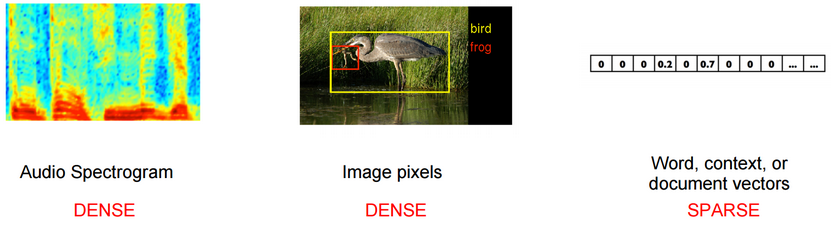
\includegraphics[scale=0.25]{pix_audio_text}
\end{frame}

%Slide-----------------------------------------------------------------------------------

\begin{frame}[t]
\frametitle{Vector representation of words (a.k.a. word embeddings)}
    Vector space models represent words in a continuous vector space, \par
    where semantically similar words are mapped to nearby points. \par
    \vspace{0.5em}
    \textbf{Distributional hypothesis:} \par
    \begin{itemize}
        \item words with similar distributions have similar meanings
        \item words in similar contexts share semantic meaning
    \end{itemize}
    \parbox[][][c]{7.5cm}{%
        \begin{enumerate}
            \item count-based methods (LSA)
            \begin{itemize}
                \item compute statistics of neighbors co-occurrences from large text corpus
                \item for each word, map statistics to a small and dense vector
            \end{itemize}
            \item predictive methods (NPL)
            \begin{itemize}
                \item predict word from neighbors using learned small and dense vectors
                \item embedding vectors are parameters of the model
            \end{itemize}
        \end{enumerate}
    }
    \parbox[][4.5cm][t]{3cm}{%
        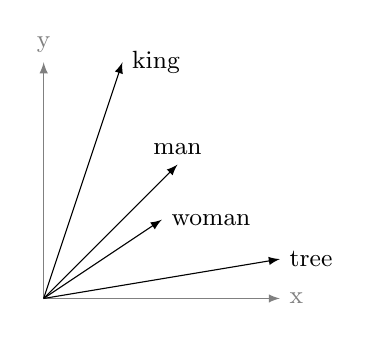
\begin{tikzpicture}
            \coordinate (Origin) at (0,0);
            \draw[gray,-latex] (Origin) -- (3,0) node [right] {\small x};
            \draw[gray,-latex] (Origin) -- (0,3) node [above] {\small y};
            \draw[-latex] (Origin) -- (1,3) node [right] {\small king};
            \draw[-latex] (Origin) -- (1.7,1.7) node [above] {\small man};
            \draw[-latex] (Origin) -- (1.5,1) node [right] {\small woman};
            \draw[-latex] (Origin) -- (3,0.5) node [right] {\small tree};
        \end{tikzpicture}
    }
    \par
\end{frame}

%Slide-----------------------------------------------------------------------------------

\begin{frame}[t]
\frametitle{Learning vector representation of words}
    Language models: \par
    \begin{itemize}
        \item Feedforward neural network
        \item Recurrent neural network
        \item Continuous bag-of-words
        \item Continuous skip-gram 
    \end{itemize}
\end{frame}

%Slide-----------------------------------------------------------------------------------

\begin{frame}[t]
\frametitle{word2vec}
    Important architecture in neural network language models \par
    Statistical approach coupled with machine learning \par
    \begin{center}
        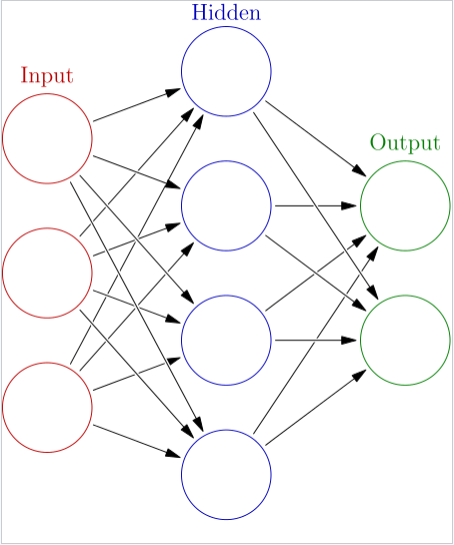
\includegraphics[scale=0.2]{nn}
    \end{center}
    \begin{itemize}
        \item Continuous bag-of-words (CBOW) 
        \item Skip-gram 
    \end{itemize}
\end{frame}

%Slide-----------------------------------------------------------------------------------

\begin{frame}[t]
\frametitle{CBOW based architecture}
    Log linear classifier with input averaged over past and future word vectors. \par
    Predicts a missing word from a given context of word sequence. \par
    \vspace{1em} 
    Example: \par
    \begin{itemize}
        \item latent Dirichlet {\bf allocation} 
    \end{itemize}
    \vspace{2em} 
  
    Useful for these cases: \par
    \begin{itemize}
        \item missing word in sentence or long phrase 
        \item meaningful bigrams $\rightarrow$ state -- capital
        \item effective sentiment orientation
    \end{itemize}
\end{frame}

%Slide-----------------------------------------------------------------------------------

\begin{frame}[t]
\frametitle{Skip-gram based architecture}
    Log linear classifier. \par
    Predicts missing context of word sequence from a given word \par
    \vspace{1em} 
    Example: \par
    \begin{itemize}
        \item {\bf latent} Dirichlet {\bf allocation}
    \end{itemize}
\end{frame}

%Slide-----------------------------------------------------------------------------------

\begin{frame}[t]
\frametitle{Vector representation of words (a.k.a. word embeddings)}
    Consider 3 sentences, vocabulary of 5 distinct words, and \par
    window size of 2 words. \par
    \begin{table}[ht]
        \centering
        \begin{tabular}{L{4cm}}
            \textbf{S1:} w1 w2 w3 \\
            \textbf{S2:} w2 w4 \\
            \textbf{S3:} w1 w5 w4 \\
        \end{tabular}
        \begin{tabular}{L{4cm}}
            \fbox{w1 w2} \fbox{w2 w3} \\
            \fbox{w2 w4} \\
            \fbox{w1 w5} \fbox{w5 w4} \\
        \end{tabular}
    \end{table}
    \vspace{-1em} 
    \begin{table}[ht]
        \centering
        \begin{tabular}{C{0.5cm}*{5}{C{0.5cm}}}
            & \textbf{w1} & \textbf{w2} & \textbf{w3} & \textbf{w4} & \textbf{w5} \\
            \cline{2-6}
            \textbf{w1} & \multicolumn{1}{|c|}{0} & \multicolumn{1}{|c|}{1} & \multicolumn{1}{|c|}{0} & \multicolumn{1}{|c|}{0} & \multicolumn{1}{|c|}{1} \\
            \cline{2-6}
            \textbf{w2} & \multicolumn{1}{|c|}{0} & \multicolumn{1}{|c|}{0} & \multicolumn{1}{|c|}{1} & \multicolumn{1}{|c|}{1} & \multicolumn{1}{|c|}{0} \\
            \cline{2-6}
            \textbf{w3} & \multicolumn{1}{|c|}{0} & \multicolumn{1}{|c|}{0} & \multicolumn{1}{|c|}{0} & \multicolumn{1}{|c|}{0} & \multicolumn{1}{|c|}{0} \\
            \cline{2-6}
            \textbf{w4} & \multicolumn{1}{|c|}{0} & \multicolumn{1}{|c|}{0} & \multicolumn{1}{|c|}{0} & \multicolumn{1}{|c|}{0} & \multicolumn{1}{|c|}{0} \\
            \cline{2-6}
            \textbf{w5} & \multicolumn{1}{|c|}{0} & \multicolumn{1}{|c|}{0} & \multicolumn{1}{|c|}{0} & \multicolumn{1}{|c|}{1} & \multicolumn{1}{|c|}{0} \\
            \cline{2-6}
        \end{tabular}
    \end{table}
    \begin{itemize}
        \item window size = $k$-words
        \item number of rows = vocabulary size 
        \item number of columns = vector dimensionality 
    \end{itemize}
\end{frame}

%Slide-----------------------------------------------------------------------------------

\begin{frame}[t]
\frametitle{CBOW Example}
    \begin{itemize}
        \item latent Dirichlet {\bf allocation} 
    \end{itemize}
    \parbox[][][b]{3cm}{%
        \tikzstyle{label} = [rectangle,outer sep=0cm,inner sep=0.08cm, text width=3cm]
        \tikzstyle{neuron} = [rectangle,draw]
        \begin{tikzpicture}[remember picture,node distance=0cm,outer sep=0cm]
            \foreach \i [count=\j] in {0,...,4}
            {
                \ifthenelse{\j=1}
                    {\node[label](l\j) {\hfill latent, $1 = x_\j$};}
                    {\ifthenelse{\j=2}
                        {\node[label,below=of l\i](l\j) {\hfill Dirichlet, $1 = x_\j$};}
                        {\node[label,below=of l\i](l\j) {\hfill$0 = x_\j$};}
                    }
            }

            \foreach \i [count=\j] in {0,...,4}
            {
                \ifthenelse{\j=1}
                    {\node[neuron,right=of l\j](w\j) {$w_\j$};}
                    {\node[neuron,below=of w\i](w\j) {$w_\j$};}
            }

            \foreach \i [count=\j] in {0,...,4}
            {
                \ifthenelse{\j=1}
                    {\node[neuron,right=of w\j,right=3.5cm](o\j) {$o_\j$};}
                    {\node[neuron,below=of o\i](o\j) {$o_\j$};}
            }

            \foreach \i [count=\j] in {0,...,2}
            {
                \ifthenelse{\j=1}
                    {\path (w2) -- (o2) node[neuron,midway](h\j) {$h_\j$};}
                    {\node[neuron,below=of h\i](h\j) {$h_\j$};}
            }

            \foreach \i in {1,...,5}
                \foreach \j in {1,...,3}
                {
                    \ifthenelse{\i=1 \AND \j=1}
                        {\draw (w\i) -- (h\j) node[above,midway](lw\i\j) {$w_{\i\j}$};}
                        {\ifthenelse{\i=5 \AND \j=3}
                            {\draw (w\i) -- (h\j) node[midway](lw\i\j) {};}
                            {\draw (w\i) -- (h\j);}
                        }
                }

            \foreach \i in {1,...,3}
                \foreach \j in {1,...,5}
                {
                    \ifthenelse{\i=1 \AND \j=1}
                        {\draw (h\i) -- (o\j) node[above,midway](lww\i\j) {$w\mrq_{\i\j}$};}
                        {\ifthenelse{\i=3 \AND \j=5}
                            {\draw (h\i) -- (o\j) node[midway](lww\i\j) {};}
                            {\draw (h\i) -- (o\j);}
                        }
                }
        \end{tikzpicture}
    }
    \par
    \hspace{2cm}
    \parbox[][3.5cm][b]{3cm}{%
        \tikzstyle{vector} = [rectangle,draw]
        \begin{tikzpicture}[remember picture,node distance=0cm,outer sep=0cm]
            \node[vector](w11) {$w_{11}$};
            \foreach \i [count=\ii] in {2,...,5}
            {
                \node[vector,below=of w\ii1](w\i1) {$w_{\i1}$};
            }
            \node[vector,right=of w11](w12) {$w_{12}$};
            \foreach \i [count=\ii] in {2,...,5}
            {
                \node[vector,below=of w\ii2](w\i2) {$w_{\i2}$};
            }
            \node[vector,right=of w12](w13) {$w_{13}$};
            \foreach \i [count=\ii] in {2,...,5}
            {
                \node[vector,below=of w\ii3](w\i3) {$w_{\i3}$};
            }

            \node[vector,right=of w23,right=0.5cm](ww11) {$w\mrq_{11}$};
            \foreach \i [count=\ii] in {2,...,5}
            {
                \node[vector,right=of ww1\ii](ww1\i) {$w\mrq_{1\i}$};
            }
            \node[vector,below=of ww11](ww21) {$w\mrq_{21}$};
            \foreach \i [count=\ii] in {2,...,5}
            {
                \node[vector,right=of ww2\ii](ww2\i) {$w\mrq_{2\i}$};
            }
            \node[vector,below=of ww21](ww31) {$w\mrq_{31}$};
            \foreach \i [count=\ii] in {2,...,5}
            {
                \node[vector,right=of ww3\ii](ww3\i) {$w\mrq_{3\i}$};
            }

            \draw[->,thick,latex-] (w12) -- (lw53) node[right=0.1cm,midway] {\small I-H weights};
            \draw[->,thick,latex-] (ww13) -- (lww35) node[right,midway] {\small H-O weights};
        \end{tikzpicture}
    }
    \par
\end{frame}

%Slide-----------------------------------------------------------------------------------

\begin{frame}[t]
    \frametitle{Training CBOW model}
    \begin{enumerate}
        \item Forward-propagation (optimization objective function)
        \item Check errors (stochastic gradient descent)
        \item Back-propagation 
    \end{enumerate}
    \vspace{0.3em}
    Perform steps 1 -- 3 until neuron weights are optimized. \par
    \vspace{-0.3em}
    \begin{itemize}
        \item initially selected from uniform random distribution $[-1, 1]$. \par
    \end{itemize}
    \vspace{0.3em}
    \hspace{2cm}
    \parbox[][][b]{3cm}{%
        \tikzstyle{neuron} = [rectangle,draw]
        \begin{tikzpicture}[node distance=0cm,outer sep=0cm]
            \foreach \i [count=\j] in {0,...,4}
            {
                \ifthenelse{\j=1}
                    {\node[neuron](w\j) {$w_\j$};}
                    {\node[neuron,below=of w\i](w\j) {$w_\j$};}
            }

            \foreach \i [count=\j] in {0,...,4}
            {
                \ifthenelse{\j=1}
                    {\node[neuron,right=of w\j,right=3.5cm](o\j) {$o_\j$};}
                    {\node[neuron,below=of o\i](o\j) {$o_\j$};}
            }

            \foreach \i [count=\j] in {0,...,2}
            {
                \ifthenelse{\j=1}
                    {\path (w2) -- (o2) node[neuron,midway](h\j) {$h_\j$};}
                    {\node[neuron,below=of h\i](h\j) {$h_\j$};}
            }

            \foreach \i in {1,...,5}
                \foreach \j in {1,...,3}
                {
                    \ifthenelse{\i=1 \AND \j=1}
                        {\draw (w\i) -- (h\j) node[above,midway](lw\i\j) {$w_{\i\j}$};}
                        {\draw (w\i) -- (h\j);}
                }

            \foreach \i in {1,...,3}
                \foreach \j in {1,...,5}
                {
                    \ifthenelse{\i=1 \AND \j=1}
                        {\draw (h\i) -- (o\j) node[above,midway](lww\i\j) {$w\mrq_{\i\j}$};}
                        {\draw (h\i) -- (o\j);}
                }

            \node[above=of w1,above=0.3cm](fp0) {};
            \node[above=of o1,above=0.3cm](fp1) {};
            \node[below=of o5,below=0.3cm](bp0) {};
            \node[below=of w5,below=0.3cm](bp1) {};
            \draw [->,-latex,thick] (fp0) -- (fp1) node [above,midway] {\textbf{Forward-propagation}};
            \node[right=of o3,right=0.3cm] {\textbf{Check errors}};
            \draw [->,-latex,thick] (bp0) -- (bp1) node [below,midway] {\textbf{Back-propagation}};
        \end{tikzpicture}
    }
    \par
\end{frame}

%Slide-----------------------------------------------------------------------------------

\begin{frame}[t]
\frametitle{Forward-propagation (input-to-hidden layer)}
    \hspace{2cm}
    \parbox[][][b]{3cm}{%
        \tikzstyle{label} = [rectangle,outer sep=0cm]
        \tikzstyle{neuron} = [rectangle,draw]
        \begin{tikzpicture}[node distance=0cm,outer sep=0cm]
            \foreach \i [count=\j] in {0,...,4}
            {
                \ifthenelse{\j=1}
                    {\node[label](l\j) {$x_\j$};}
                    {\node[label,below=of l\i](l\j) {$x_\j$};}
            }

            \foreach \i [count=\j] in {0,...,4}
            {
                \ifthenelse{\j=1}
                    {\node[neuron,right=of l\j](w\j) {$w_\j$};}
                    {\node[neuron,below=of w\i](w\j) {$w_\j$};}
            }

            \foreach \i [count=\j] in {0,...,4}
            {
                \ifthenelse{\j=1}
                    {\node[lightgray,neuron,right=of w\j,right=3.5cm](o\j) {$o_\j$};}
                    {\node[lightgray,neuron,below=of o\i](o\j) {$o_\j$};}
            }

            \foreach \i [count=\j] in {0,...,2}
            {
                \ifthenelse{\j=1}
                    {\path (w2) -- (o2) node[neuron,midway](h\j) {$h_\j$};}
                    {\node[neuron,below=of h\i](h\j) {$h_\j$};}
            }

            \foreach \i in {1,...,5}
                \foreach \j in {1,...,3}
                {
                    \ifthenelse{\i=1 \AND \j=1}
                        {\draw (w\i) -- (h\j) node[above,midway](lw\i\j) {$w_{\i\j}$};}
                        {\draw (w\i) -- (h\j);}
                }

            \foreach \i in {1,...,3}
                \foreach \j in {1,...,5}
                {
                    \ifthenelse{\i=1 \AND \j=1}
                        {\draw[lightgray] (h\i) -- (o\j) node[above,midway](lww\i\j) {$w\mrq_{\i\j}$};}
                        {\draw[lightgray] (h\i) -- (o\j);}
                }
        \end{tikzpicture}
    }
    \par
    \parbox[][3cm][c]{5.5cm}{%
        $\mathbf{h = W^Tx}$ \par
        $h_1 = (w_{11}x_1 + w_{21}x_2 + \dots + w_{51}x_5)$ \par
        $h_2 = (w_{12}x_1 + w_{22}x_2 + \dots + w_{52}x_5)$ \par
        $h_3 = (w_{13}x_1 + w_{23}x_2 + \dots + w_{53}x_5)$
    }
    \hspace{0.5cm}
    \parbox[][3cm][c]{3cm}{%
        \tikzstyle{vector} = [rectangle,draw]
        \begin{tikzpicture}[node distance=0cm,outer sep=0cm]
            \node[vector](w11) {$w_{11}$};
            \foreach \i [count=\ii] in {2,...,5}
            {
                \node[vector,right=of w\ii1](w\i1) {$w_{\i1}$};
            }
            \node[vector,below=of w11](w12) {$w_{12}$};
            \foreach \i [count=\ii] in {2,...,5}
            {
                \node[vector,right=of w\ii2](w\i2) {$w_{\i2}$};
            }
            \node[vector,below=of w12](w13) {$w_{13}$};
            \foreach \i [count=\ii] in {2,...,5}
            {
                \node[vector,right=of w\ii3](w\i3) {$w_{\i3}$};
            }

            \node[vector,right=of w51,right=0.3cm](l3) {$x_3$};
            \node[vector,above=of l3](l2) {$x_2$};
            \node[vector,above=of l2](l1) {$x_1$};
            \node[vector,below=of l3](l4) {$x_4$};
            \node[vector,below=of l4](l5) {$x_5$};

        \end{tikzpicture}
    }
    \par
\end{frame}

%Slide-----------------------------------------------------------------------------------

\begin{frame}[t]
\frametitle{Forward-propagation (hidden-to-output layer)}
    \hspace{2cm}
    \parbox[][][b]{3cm}{%
        \tikzstyle{label} = [rectangle,outer sep=0cm]
        \tikzstyle{neuron} = [rectangle,draw]
        \begin{tikzpicture}[node distance=0cm,outer sep=0cm]
            \foreach \i [count=\j] in {0,...,4}
            {
                \ifthenelse{\j=1}
                    {\node[lightgray,label](l\j) {$x_\j$};}
                    {\node[lightgray,label,below=of l\i](l\j) {$x_\j$};}
            }

            \foreach \i [count=\j] in {0,...,4}
            {
                \ifthenelse{\j=1}
                    {\node[lightgray,neuron,right=of l\j](w\j) {$w_\j$};}
                    {\node[lightgray,neuron,below=of w\i](w\j) {$w_\j$};}
            }

            \foreach \i [count=\j] in {0,...,4}
            {
                \ifthenelse{\j=1}
                    {\node[neuron,right=of w\j,right=3.5cm](o\j) {$o_\j$};}
                    {\node[neuron,below=of o\i](o\j) {$o_\j$};}
            }

            \foreach \i [count=\j] in {0,...,2}
            {
                \ifthenelse{\j=1}
                    {\path (w2) -- (o2) node[neuron,midway](h\j) {$h_\j$};}
                    {\node[neuron,below=of h\i](h\j) {$h_\j$};}
            }

            \foreach \i in {1,...,5}
                \foreach \j in {1,...,3}
                {
                    \ifthenelse{\i=1 \AND \j=1}
                        {\draw[lightgray] (w\i) -- (h\j) node[above,midway](lw\i\j) {$w_{\i\j}$};}
                        {\draw[lightgray] (w\i) -- (h\j);}
                }

            \foreach \i in {1,...,3}
                \foreach \j in {1,...,5}
                {
                    \ifthenelse{\i=1 \AND \j=1}
                        {\draw (h\i) -- (o\j) node[above,midway](lww\i\j) {$w\mrq_{\i\j}$};}
                        {\draw (h\i) -- (o\j);}
                }
        \end{tikzpicture}
    }
    \par
    \vspace{1em}
    \parbox[][3cm][c]{6.9cm}{%
        $\mathbf{Net(O) = u = W\mrq^Th}$ \par
        $Net(o_1) = u_1 = (w\mrq_{11}h_1 + w\mrq_{21}h_2 + w\mrq_{31}h_3)$ \par
        $Net(o_2) = u_2 = (w\mrq_{12}h_1 + w\mrq_{22}h_2 + w\mrq_{32}h_3)$
        $$\vdots$$
        $Net(o_5) = u_5 = (w\mrq_{15}h_1 + w\mrq_{25}h_2 + w\mrq_{35}h_3)$
    }
    \hspace{0.5cm}
    \parbox[][3cm][c]{3cm}{%
        \tikzstyle{vector} = [rectangle,draw]
        \begin{tikzpicture}[node distance=0cm,outer sep=0cm]
            \node[vector](ww11) {$w\mrq_{11}$};
            \foreach \i [count=\ii] in {2,...,5}
            {
                \node[vector,below=of ww1\ii](ww1\i) {$w\mrq_{1\i}$};
            }
            \node[vector,right=of ww11](ww21) {$w\mrq_{21}$};
            \foreach \i [count=\ii] in {2,...,5}
            {
                \node[vector,below=of ww2\ii](ww2\i) {$w\mrq_{2\i}$};
            }
            \node[vector,right=of ww21](ww31) {$w\mrq_{31}$};
            \foreach \i [count=\ii] in {2,...,5}
            {
                \node[vector,below=of ww3\ii](ww3\i) {$w\mrq_{3\i}$};
            }

            \node[vector,right=of ww32,right=0.3cm](h1) {$h_1$};
            \node[vector,below=of h1](h2) {$h_2$};
            \node[vector,below=of h2](h3) {$h_3$};

        \end{tikzpicture}
    }
    \par
\end{frame}

%Slide-----------------------------------------------------------------------------------

\begin{frame}[t]
\frametitle{Forward-propagation (softmax classifier)}
    $$Out(o_1) = y_1 = \frac{e^{u_1}}{e^{u_1} + e^{u_2} + \dots + e^{u_5}}$$
    $$Out(o_2) = y_2 = \frac{e^{u_2}}{e^{u_1} + e^{u_2} + \dots + e^{u_5}}$$
    $$\vdots$$
    $$Out(o_5) = y_5 = \frac{e^{u_5}}{e^{u_1} + e^{u_2} + \dots + e^{u_5}}$$
    \par\vspace{1em}
    Softmax output for word $w_j$ w.r.t. context $w_I$ $\rightarrow$ conditional probability
    $$\mathbf{P(w_j \rvert w_I) = y_j = \frac{e^{u_j}}{\sum_{j\mrq=1}^{V} e^{u_{j\mrq}}}}$$
\end{frame}

%Slide-----------------------------------------------------------------------------------

\begin{frame}[t]
\frametitle{Check errors}
    Assume: \par
    \begin{itemize}
        \item $w_o = $ output word
        \item $w_I = $ context words
        \item $V = $ size of input context
    \end{itemize}
    $$max\ P(w_o \rvert w_I) = max(y_{j^*}) = max(log(y_{j^*}))$$
    where $j^* =$ index of output word \par
    \vspace{1em}
    \textbf{Example:} \par
    \vspace{-1.5em}
    \begin{align*}
        E(o_4) &= log(P(w_{o_4} \rvert w_I)) = log_e\left(\frac{e^{u_j}}{\sum_{j\mrq=1}^{V} e^{u_{j\mrq}}}\right) \\
               &= u_4 - log_e\left(\sum_{j\mrq=1}^{V} e^{u_{j\mrq}}\right)
    \end{align*}
\end{frame}

%Slide-----------------------------------------------------------------------------------

\begin{frame}[t]
\frametitle{Check errors}
    To minimize errors, $ E = -log(P(w_o \rvert w_I))$ \par
    $$E = log\left(\sum_{j\mrq=1}^{V} e^{u_{j\mrq}}\right) - u_{j^*}$$
    Derivate of $E$ w.r.t. $u_4$, \par
    $$\frac{dE(o_4)}{d(u_4)} = Out(o_4) - \frac{du_4}{du_4} = y_4 - 1$$
    \begin{equation*}
        \frac{dE}{dj} = y_j - t_j = e_j
        \begin{cases}
            \ t_j = 1,\ if\ t_j = t_{j^*} \\
            \ t_j = 0,\ otherwise  \\
        \end{cases}
    \end{equation*}
\end{frame}

%Slide-----------------------------------------------------------------------------------

\begin{frame}[t]
\frametitle{Backward-propagation (output-to-hidden layer)}
    Take gradient of $E$, w.r.t. $w\mrq_{11}$ \par
    $$\frac{dE(o_1)}{dw\mrq_{11}} = \frac{dE(o_1)}{du_1} \times \frac{du_1}{dw\mrq_{11}}$$
    \vspace{-1em}
    \begin{align*}
        \frac{dE(o_1)}{du_1} &= y_1 - 0 = e_1 \\
        \frac{du_1}{dw\mrq_{11}} &= \frac{d(w\mrq_{11}h_1 + w\mrq_{21}h_2 + w\mrq_{31}h_3)}{dw\mrq_{11}} = h_1
    \end{align*}
    $$\mathbf{\frac{dE(o_1)}{dw\mrq_{11}} = e_1 \times h_1}$$ 
    Update weight of $w\mrq_{11}$: \par
    \vspace{-1em}
    $$\mathbf{(w\mrq_{11})^{new} = w\mrq_{11} - \eta(e_1 \times h_1)}$$
    $\eta = [0,1] \rightarrow$ learning rate \par
    Need to update all neurons $w\mrq_{ij}$ \par 
\end{frame}

%Slide-----------------------------------------------------------------------------------

\begin{frame}[t]
\frametitle{Backward-propagation (hidden-to-input layer)}
    Take gradient of $E$, w.r.t. $w_{11}$ \par
    $$\frac{dE}{dw_{11}} = \frac{dE}{dh_1} \times \frac{dh_1}{dw_{11}}$$
    \vspace{-1em}
    \begin{align*}
        \frac{dE}{dh_1} &= \left(\frac{dE}{du_1} \times \frac{du_1}{dh_1}\right) + \dots + \left(\frac{dE}{du_5} \times \frac{du_5}{dh_1}\right)
        = (e_1w\mrq_{11}) + \dots + (e_5w\mrq_{15}) \\
        \frac{dh_1}{dw_{11}} &= \frac{d(w_{11}x_1 + w_{21}x_2 + \dots + w_{31}x_3)}{dw_{11}}
    \end{align*}
    $$\mathbf{\frac{dE}{dw_{11}} = x_1\frac{dE}{dh_1}}$$ 
    Update weight of $w_{11}$: \par
    \vspace{-1em}
    $$\mathbf{(w_{11})^{new} = w_{11} - \eta\frac{dE}{dw_{11}}}$$
    $\eta = [0,1] \rightarrow$ learning rate \par
    Need to update all neurons $w_{ij}$ \par 
\end{frame}

%Slide-----------------------------------------------------------------------------------

\begin{frame}[t]
\frametitle{Training optimizations}
    \textbf{Problem:} neural network is huge \par
    \begin{itemize}
        \item two weight matrices (hidden and output layers)
        \item $10K$ words $\times$ $300$ size embedding vectors = $\frac{3\ G\ weights}{matrix}$
        \item need large amount of training data to tune weights
        \item training and gradient descent are slow on such NN
    \end{itemize}
\end{frame}

%Slide-----------------------------------------------------------------------------------

\begin{frame}[t]
\frametitle{Training optimizations}
    \textbf{Solutions:} \par
    \begin{itemize}
        \item remove words that occur less than some minimum
        \item treat common pairs or phrases as single ``words" - Boston Globe
        \item subsampling frequent words to decrease number of training examples
          $$P(w_i) = \left(\sqrt{\frac{z(w_i)}{0.001}} + 1\right) \times \frac{0.001}{z(w_i)}$$
          $w_i$ is a word, $z(w_i)$ is $w_i$ frequency in corpus,
          $P(w_i)$ is the probability of keeping $w_i$ \par
    \end{itemize}
\end{frame}

%Slide-----------------------------------------------------------------------------------

\begin{frame}[t]
\frametitle{Training optimizations}
    \textbf{Solutions:} \par
    \begin{itemize}
        \item modify the optimization objective function
        \begin{itemize}
            \item negative sampling - Each training sample updates some weights.
                  Negative samples are chosen from a ``unigram distribution".
                  The probability for selecting a word is related to its frequency.
              $$P(w_i) = \frac{f(w_i)^{3/4}}{\sum_{j=0}^{n} f(w_j)^{3/4}}$$
            \item hierarchical softmax layers - reduce output layer to $log_2|V|$
        \end{itemize}
    \end{itemize}
\end{frame}

%Slide-----------------------------------------------------------------------------------

\begin{frame}
    \centering THE END
\end{frame}

%----------------------------------------------------------------------------------------

\end{document}
%----------------------------------------------------------------------------------------

